% vim:set et sw=2 ts=4 tw=72:
% Jun 24, 2017

\dmg{don't editorialize: simply say: the results show that Linvis is superior to ... in ....
as we discussed today, it is about the tools more than the model
}

Overall, the results show fairly conclusive results; the DAG is unable
to adequately provide users with an explanation of the changes being
made in the repository, the DAG is not easily understood, and the DAG is
unable to provide summarizations of the changes being made at a merge.
Meanwhile, the \mt model is able to provide a better explanation of how
a commit is integrated, along with better summarization capabilities. In
this section, we discuss some observations made during the study,
threats to the validity of the study, comments made by the participants
during the study, modifications to the original algorithm to help
generalize it for more repositories, and future work.

\subsection{Observations}
\label{sub:observations}

% TODO: include info on merge tree sizes

\dmg{I think you mean challenge using gitk, right? so be explicit}

During the course of the study, we noticed a consistent theme among the
participants. The most difficult challenge was identifying the master
branch of the repository. Given that single-commit merge trees are the
most common tree, and that they are relatively simple, we were
interested in seeing if the participants would be able to identify the
tree easily, but the results suggest that this was not the case.
\dmg{the following is hard to understand. even i don't quite get what you mean}
The
issue primarily stemmed from not being able to identify the master
branch. Most of the participants realized that they should not be going
backward, toward the initial commit, very early on. Furthermore, many
would identify the correct commit; however, they would start listing
every merge along the master branch as being a merge in the tree, and
including the commits from that merge. In the case of the single commit,
simply identifying the master branch would most likely be sufficient in
providing a clearer understanding of how a commit or flat tree is
integrated into the master branch of the repository.

While, in general, the participants of the study preferred using \tool
to Gitk, there were some noticeable usability issues. The most prominent
issue being the navigation within the tree. The participants expected
that the tabs would update when they clicked on a node in the tree,
instead of having to click the link to the commit after clicking the
node. This was true in both the Reingold-Tilford tree and the Pack tree.
The second major usability issue was the inconsistency between the list
tree and the other tree visualizations. The list tree is rooted at the
repository event that the user is current looking at, while the other
tree visualizations show the entire tree, and use bright orange to
highlight the current node.


\subsection{Comments From a Release Manager}
\label{sub:comments_from_a_release_manager}

One of the participants of the study had worked as a release manager for
more than three years, working with both SVN and CVS repositories, but
had little experience with git.

Contributors making merges need to understand more than just what merges
a commit was collected into before reaching the repository of the
contributor. It is also important to understand order that the related
commits were made, as they tell the story of what the developer was
thinking as they were writing the changes. The current merge-tree model
does not order the commits, simply placing them randomly. This is the
primary reason behind this participant's request to use both
simultaneously. \tool is able to help with the aggregation of the
information, and provide a better understanding of the next merge
involved in integrating this commit, but the DAG in gitk provides the
full story of the commit instead of hiding it behind a layer of
abstraction.

The comments from this participant were very insightful, and will assist
in improving the model in the future.

\subsection{Threats to Validity}
\label{sub:threats}

\dmg{divide it onto internal and external validity: internal: the tasks were only two merges, but they
were randomnly chosen to be representative; the tasks were randomized to avoid bias, few participants, 
but statistical analysis used to measure significance}

\dmg{regarding external, as you say, participants might not be experts, since they are students,
  you compared against git and gitk (part of git) because they are the most default tools everybody uses
  but other tools or version control systems might provide better summarizations --i don't know of any.
}


While git includes gitk and the git log provides a view of the DAG with
\verb|git log --graph|, many of the participants in our study were
unfamiliar with the DAG visualizations shown by these tools. A possible
reason for this may be that unless a repository reaches a sufficient
complexity, both in branching and number of commits, these tools are
necessary for the normal operation of git. Furthermore, fear of the
complexity caused by branching may cause personal and academic
repositories to have relatively simple structures. While they were
unfamiliar with the DAG structure, these users were also unfamiliar with
the \mt model, and were still able to better understand and summarize
the repository using \tool.

\dmg{this paragraph i don't get:}
Each question was evaluated independently of the results from the
previous question in the summarization tasks. Had we modified the
correct answer to fit the conceptual understanding of which commits were
included in the tree, we may have witnessed different results. A
modification to the study may include providing the participants with
the correct set of commits prior to the summarization tasks, after the
merge task set.

\subsection{Generalization}
\label{sub:generalization}

Seeing that the \mt model is able to assist users with understanding how
commits are integrated, we continue by looking at ways of improving the
algorithm for faster operations, and making the conversion from DAG to
\mt feasible over the internet for smaller repositories.

The problem of identifying the master branch is the most difficult, and is
not possible without heuristic approaches. The master branch can be
confounded by \textit{foxtrot} merges, which change the order of the
parents in the parent list of a merge. Other than the ordering of the
parent list, git has no other way to determine which commits are on the
master branch of the repository. For the purpose of this discussion, we
will assume that we can rely on the order of the parent list to be
correct, and that foxtrots do not occur.

\begin{algorithm}
  \caption{Computing the generalized Merge Tree}
  \label{alg:generalized}
  \begin{algorithmic}[1]
    \Function{Phase 1}{initial commit $root$} : updated tree
    \State $depth \gets 0$
    \State $Q \gets root$
    \Do
    \State $cur \gets Q.dequeue$
    \State $parents \gets cur.parents$
    \State $depth \gets depth + parents.length - 1$
    \For{$index, parent \in parents$}
    \If{$parent.depth$ is $undefined$}
    \State $parent.depth \gets cur.depth + index$
    \ElsIf {$cur.depth > parent.depth$}
    \State $depth \gets depth - 1$
    \ElsIf {$cur.depth < parent.depth$}
    \State $depth \gets depth - 1$
    \State $parent.depth \gets cur.depth$
    \EndIf
    \State $parent.children \gets cur$
    \If{$parent$ has not been visited}
    \State $Q \gets parent$
    \State $parent.visited \gets True$
    \EndIf
    \EndFor
    \doWhile{$Q$ not empty and $depth \ne 0$ }
    \EndFunction

    \Function{Phase 2}{initial commit $root$} : Merge tree
    \State $tree.root \gets root$
    \State $Q$ // Empty Queue

    \State $parents \gets root.parents$
    \State $parents \gets tail\ parents$
    \For {$parent \in parents$}
    \State $realParent \gets min(\forall child \in parent.children,\ parent.depth >= child.depth)$
    \If {$realParent$ is $root$}
    \State $root.children \gets parent$
    \State $parent.parent \gets root$
    \State $Q \gets parent$
    \EndIf
    \EndFor

    \While{$Q$ not empty}
    \State $cur \gets Q.dequeue$
    \State $parents \gets cur.parents$
    \For{$parent \in parents$}
    \State $realParent \gets min(\forall child \in parent.children,\ parent.depth >= child.depth)$
    \If {$realParent$ is $cur$}
    \State $cur.children \gets parent$
    \State $parent.parent \gets cur$
    \State $Q \gets parent$
    \EndIf

    \EndFor
    \EndWhile

    \EndFunction
  \end{algorithmic}
\end{algorithm}

The primary difference between the original algorithm and the
generalization is the main data structure. Algorithm~\ref{alg:original}
is centered around the use of the stack, making it akin to a depth-first
traversal of the DAG.\@ The generalization in
Algorithm~\ref{alg:generalized} is based on the queue, making it akin to
the breadth-first traversal of the DAG.\@ While the final results of the
two traversals should not be different, the runtime properties are
different.

We will begin with a simplified description of the original algorithm.
We start at the master branch pointer. We will use the term master
branch loosely here, meaning any branch that has been labeled in some
way as being the main branch, this branch may have a different name, but
standard naming conventions call it the master branch. Starting from the
master branch label, we traverse the entire master branch to the initial
commit, recording the commit hash of every repository event encountered.

The second phase iterates over every commit, computing the shortest
distance to the master branch. For this reason, the entire repository
must be available to the algorithm. This is a dynamic programming
solution, centered around the call stack. The next node on the shortest
path to the master branch will become the parent of this node in the
tree.

If this algorithm is to be generalized into a dynamic, web-based, tool,
it may not be feasible to download every commit in the repository in a
reasonable period of time. We instead look toward a breadth-first
approach at limiting the number of repository events that must be
downloaded.

Focusing on the generalized algorithm~\ref{alg:generalized}, the
algorithm is broken into two phases. The first phase is where the
improvements take place. The first phase has three main goals, the first
is to track the master branch. The second goal labels the depth of each
repository event that is traverses. The final goal is to record the
children of each commit, reversing the DAG.\@ The first phase also
begins the process of reversing the DAG, by providing the candidate
commits that could possibly be the real parent to this node. The first
phase can terminate early, if it reaches a point where all branches that
it is following terminate. The depth metric on line 7 indicates how many
branches are currently being traversed. In line 11 through 15, we
decrement the depth, as this is the point where a branch occurs. The
changing of the depth occurs if there are more events on the same branch
than between the merge and branch point of a separate branch.

\begin{table}[htpb]
  \centering
  \caption{Example traversal of the example DAG in
    Figure~\ref{fig:repoDAG} starting at merge 11.}
  \label{tab:ex_traversal}
  \begin{tabular}{cccc|cc}
    \toprule
    Current & Parents & Depth & Q       & Visited & Children\\\midrule
    -       & -       & 0     & 11      & 11:0    & \\
    11      & 4,9     & 1     & 4,9     & 4:0     & 11, 5\\
    4       & 1       & 1     & 9,1     & 9:1     & 11\\
    9       & 7,6,8   & 3     & 1,7,6,8 & 7:1     & 9, 8\\
    1       &         & 3     & 7,6,8   & 6:2     & 9\\
    7       & 5       & 3     & 6,8,5   & 8:3     & 9\\
    6       & 5       & 2     & 8,5     & 5:1     & 7, 6\\
    8       & 7       & 1     & 5       & 2:1     & 5, 3\\
    5       & 4,2,3   & 2     & 2,3     & 3:2     & 5\\
    2       & 1       & 1     & 3       &         & \\
    3       & 2       & 0     &         &         & \\
    \bottomrule
  \end{tabular}
\end{table}

In Table~\ref{tab:ex_traversal}, we follow the algorithm starting at
merge commit 11 from the example in Figure~\ref{fig:repoDAG}, recording
the current node, the parents of the current node, the depth after
updating, and the queue structure after updating. The visited column is
not dependant on the current step, but keeps track of the nodes that
have been visited, and the depth at that node. When we reverse the DAG,
the children in this table will become the candidates for being the
parent of the corresponding node. For example, the parent of node 7 may
be resolved to either node 9 or node 8. In this case, the shortest path
to the master branch is through node 9.

The terminology surrounding the parent/child relationship gets very
confusing at the change between phase one and two because this is where
the roles switch. In phase 1, we are working with the DAG; in phase 2,
we are working with a structure that is neither a tree nor a DAG, but
can only be described as a directed graph.

The goal of the second phase is to resolve the tree from the directed
graph. We will refer to parents in the same sense as we would refer to
them in the tree form of the repository for the remainder of this
section. We have gathered the depths and possible parents (line 17), but
we need to remove the extra parents. Extra parents are culled in line
42 of the algorithm. Of the possible parents, we take the parent that is
closest to the root, but not beyond. This forces the real parent to
either be deeper in the tree, or on the same branch. Line 30 to 37 are
for bootstrapping the queue, ensuring that we are not starting on an
empty queue.

The construction of the tree becomes trivial now that we are able to
determine the parents and children for each node. Lines 44 and 45
perform this construction, adding the DAG parent to the tree children of the
current node, and the DAG parent's parent becomes the current node,
which was the DAG parent's child. We continue following the path until
we hit the root node, merging the commit into the master branch.

This algorithm relies heavily on the order of parents in the parent
list, but is able to trim the number of nodes that must be downloaded.
Furthermore, the resulting tree is able to show the order of commits,
telling the story of how a developer was working, before the set of
commits was merged. We developed a small bitbucket plugin to test the
design and determine whether it was capable of producing merge trees,
shown in Figure~\ref{fig:b_plugin}.

\begin{figure}[htpb]
  \centering
  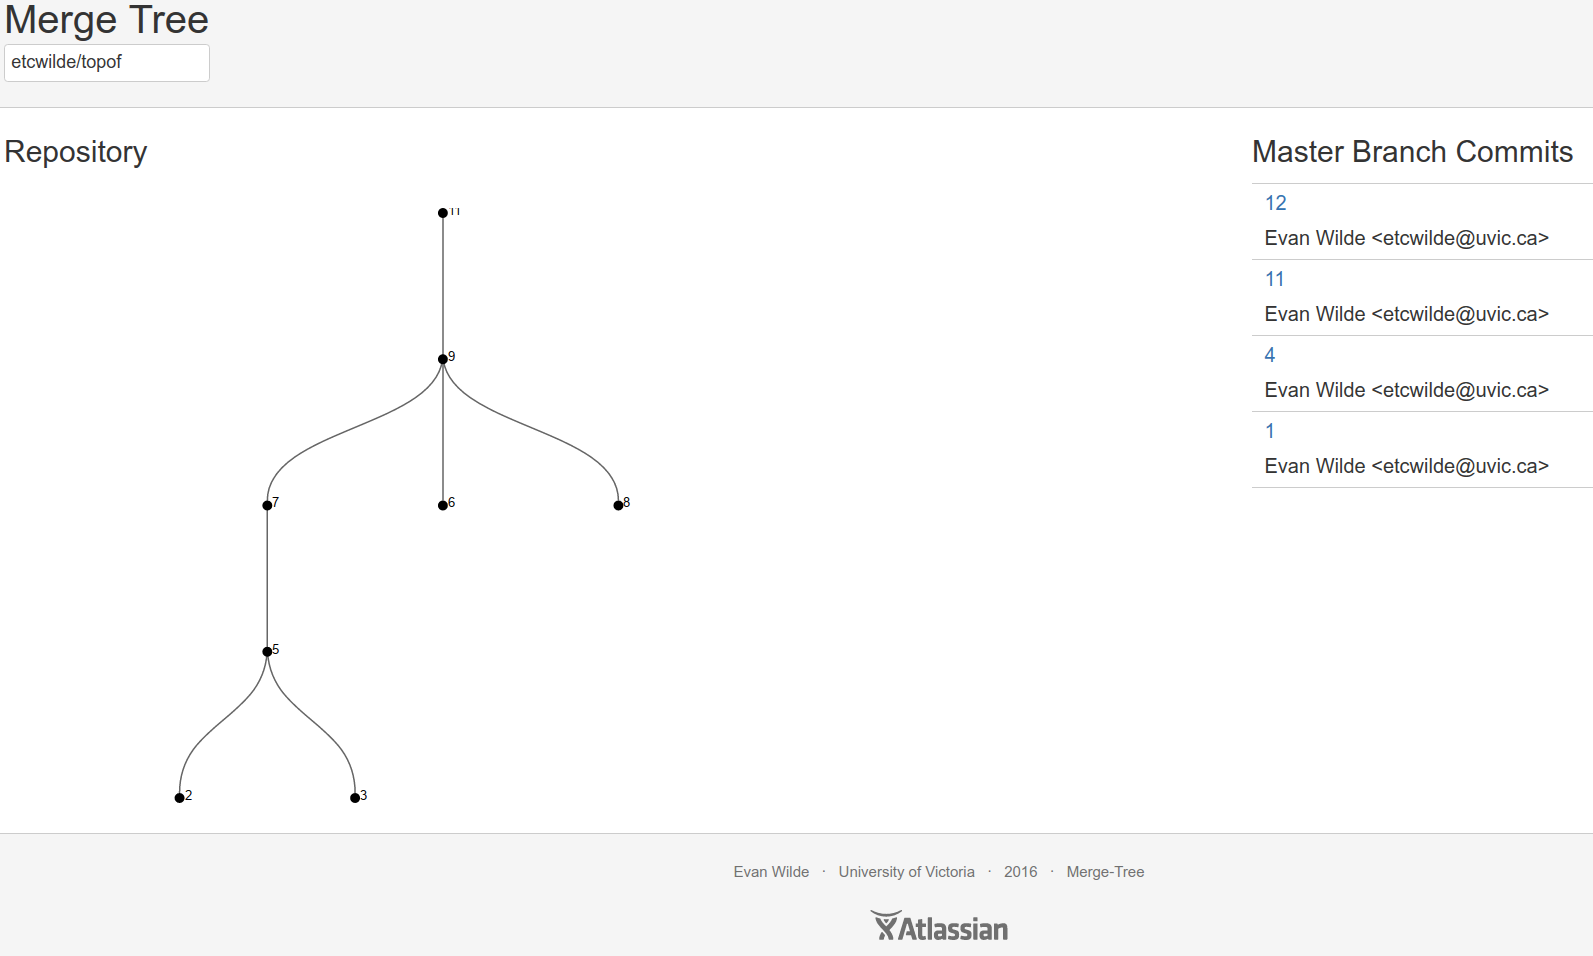
\includegraphics[width=\linewidth]{figures/plugin.png}
  \caption{Screen shot of the Bitbucket plugin showing the online tree
    computation of the repository shown in~\ref{fig:repoDAG}.}
  \label{fig:b_plugin}
\end{figure}


%%% Local Variables:
%%% mode: latex
%%% TeX-master: "userstudy"
%%% End:
